\documentclass[twoside]{book}

% Packages required by doxygen
\usepackage{fixltx2e}
\usepackage{calc}
\usepackage{doxygen}
\usepackage[export]{adjustbox} % also loads graphicx
\usepackage{graphicx}
\usepackage[utf8]{inputenc}
\usepackage{makeidx}
\usepackage{multicol}
\usepackage{multirow}
\PassOptionsToPackage{warn}{textcomp}
\usepackage{textcomp}
\usepackage[nointegrals]{wasysym}
\usepackage[table]{xcolor}

% Font selection
\usepackage[T1]{fontenc}
\usepackage[scaled=.90]{helvet}
\usepackage{courier}
\usepackage{amssymb}
\usepackage{sectsty}
\renewcommand{\familydefault}{\sfdefault}
\allsectionsfont{%
  \fontseries{bc}\selectfont%
  \color{darkgray}%
}
\renewcommand{\DoxyLabelFont}{%
  \fontseries{bc}\selectfont%
  \color{darkgray}%
}
\newcommand{\+}{\discretionary{\mbox{\scriptsize$\hookleftarrow$}}{}{}}

% Page & text layout
\usepackage{geometry}
\geometry{%
  a4paper,%
  top=2.5cm,%
  bottom=2.5cm,%
  left=2.5cm,%
  right=2.5cm%
}
\tolerance=750
\hfuzz=15pt
\hbadness=750
\setlength{\emergencystretch}{15pt}
\setlength{\parindent}{0cm}
\setlength{\parskip}{3ex plus 2ex minus 2ex}
\makeatletter
\renewcommand{\paragraph}{%
  \@startsection{paragraph}{4}{0ex}{-1.0ex}{1.0ex}{%
    \normalfont\normalsize\bfseries\SS@parafont%
  }%
}
\renewcommand{\subparagraph}{%
  \@startsection{subparagraph}{5}{0ex}{-1.0ex}{1.0ex}{%
    \normalfont\normalsize\bfseries\SS@subparafont%
  }%
}
\makeatother

% Headers & footers
\usepackage{fancyhdr}
\pagestyle{fancyplain}
\fancyhead[LE]{\fancyplain{}{\bfseries\thepage}}
\fancyhead[CE]{\fancyplain{}{}}
\fancyhead[RE]{\fancyplain{}{\bfseries\leftmark}}
\fancyhead[LO]{\fancyplain{}{\bfseries\rightmark}}
\fancyhead[CO]{\fancyplain{}{}}
\fancyhead[RO]{\fancyplain{}{\bfseries\thepage}}
\fancyfoot[LE]{\fancyplain{}{}}
\fancyfoot[CE]{\fancyplain{}{}}
\fancyfoot[RE]{\fancyplain{}{\bfseries\scriptsize Generated by Doxygen }}
\fancyfoot[LO]{\fancyplain{}{\bfseries\scriptsize Generated by Doxygen }}
\fancyfoot[CO]{\fancyplain{}{}}
\fancyfoot[RO]{\fancyplain{}{}}
\renewcommand{\footrulewidth}{0.4pt}
\renewcommand{\chaptermark}[1]{%
  \markboth{#1}{}%
}
\renewcommand{\sectionmark}[1]{%
  \markright{\thesection\ #1}%
}

% Indices & bibliography
\usepackage{natbib}
\usepackage[titles]{tocloft}
\setcounter{tocdepth}{3}
\setcounter{secnumdepth}{5}
\makeindex

% Hyperlinks (required, but should be loaded last)
\usepackage{ifpdf}
\ifpdf
  \usepackage[pdftex,pagebackref=true]{hyperref}
\else
  \usepackage[ps2pdf,pagebackref=true]{hyperref}
\fi
\hypersetup{%
  colorlinks=true,%
  linkcolor=blue,%
  citecolor=blue,%
  unicode%
}

% Custom commands
\newcommand{\clearemptydoublepage}{%
  \newpage{\pagestyle{empty}\cleardoublepage}%
}

\usepackage{caption}
\captionsetup{labelsep=space,justification=centering,font={bf},singlelinecheck=off,skip=4pt,position=top}

%===== C O N T E N T S =====

\begin{document}

% Titlepage & ToC
\hypersetup{pageanchor=false,
             bookmarksnumbered=true,
             pdfencoding=unicode
            }
\pagenumbering{roman}
\begin{titlepage}
\vspace*{7cm}
\begin{center}%
{\Large My Project }\\
\vspace*{1cm}
{\large Generated by Doxygen 1.8.11}\\
\end{center}
\end{titlepage}
\clearemptydoublepage
\tableofcontents
\clearemptydoublepage
\pagenumbering{arabic}
\hypersetup{pageanchor=true}

%--- Begin generated contents ---
\chapter{File Index}
\section{File List}
Here is a list of all files with brief descriptions\+:\begin{DoxyCompactList}
\item\contentsline{section}{\hyperlink{Lab1_8c}{Lab1.\+c} }{\pageref{Lab1_8c}}{}
\end{DoxyCompactList}

\chapter{File Documentation}
\hypertarget{LUDecomp_8cpp}{}\section{L\+U\+Decomp.\+cpp File Reference}
\label{LUDecomp_8cpp}\index{L\+U\+Decomp.\+cpp@{L\+U\+Decomp.\+cpp}}
{\ttfamily \#include $<$iostream$>$}\\*
{\ttfamily \#include $<$cstdio$>$}\\*
Include dependency graph for L\+U\+Decomp.\+cpp\+:
\nopagebreak
\begin{figure}[H]
\begin{center}
\leavevmode
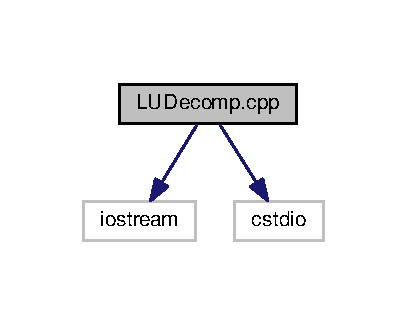
\includegraphics[width=196pt]{LUDecomp_8cpp__incl}
\end{center}
\end{figure}
\subsection*{Functions}
\begin{DoxyCompactItemize}
\item 
int \hyperlink{LUDecomp_8cpp_a3c04138a5bfe5d72780bb7e82a18e627}{main} (int argc, char $\ast$$\ast$argv)
\item 
void \hyperlink{LUDecomp_8cpp_ae9c4a9a6c6d420e1df3fed70f4faf375}{lu} (float a\mbox{[}$\,$\mbox{]}\mbox{[}10\mbox{]}, float l\mbox{[}$\,$\mbox{]}\mbox{[}10\mbox{]}, float u\mbox{[}$\,$\mbox{]}\mbox{[}10\mbox{]}, int n)
\item 
void \hyperlink{LUDecomp_8cpp_a03c4f4fac92a1c3266ad7002a68b4610}{output} (float x\mbox{[}$\,$\mbox{]}\mbox{[}10\mbox{]}, int n)
\end{DoxyCompactItemize}


\subsection{Function Documentation}
\index{L\+U\+Decomp.\+cpp@{L\+U\+Decomp.\+cpp}!lu@{lu}}
\index{lu@{lu}!L\+U\+Decomp.\+cpp@{L\+U\+Decomp.\+cpp}}
\subsubsection[{\texorpdfstring{lu(float a[][10], float l[][10], float u[][10], int n)}{lu(float a[][10], float l[][10], float u[][10], int n)}}]{\setlength{\rightskip}{0pt plus 5cm}void lu (
\begin{DoxyParamCaption}
\item[{float}]{a\mbox{[}$\,$\mbox{]}\mbox{[}10\mbox{]}, }
\item[{float}]{l\mbox{[}$\,$\mbox{]}\mbox{[}10\mbox{]}, }
\item[{float}]{u\mbox{[}$\,$\mbox{]}\mbox{[}10\mbox{]}, }
\item[{int}]{n}
\end{DoxyParamCaption}
)}\hypertarget{LUDecomp_8cpp_ae9c4a9a6c6d420e1df3fed70f4faf375}{}\label{LUDecomp_8cpp_ae9c4a9a6c6d420e1df3fed70f4faf375}

\begin{DoxyCode}
30 \{
31     \textcolor{keywordtype}{int} i = 0, j = 0, k = 0;
32     \textcolor{keywordflow}{for} (i = 0; i < n; i++)
33     \{
34         \textcolor{keywordflow}{for} (j = 0; j < n; j++)
35         \{
36             \textcolor{keywordflow}{if} (j < i)
37                 l[j][i] = 0;
38             \textcolor{keywordflow}{else}
39             \{
40                 l[j][i] = a[j][i];
41                 \textcolor{keywordflow}{for} (k = 0; k < i; k++)
42                 \{
43                     l[j][i] = l[j][i] - l[j][k] * u[k][i];
44                 \}
45             \}
46         \}
47         \textcolor{keywordflow}{for} (j = 0; j < n; j++)
48         \{
49             \textcolor{keywordflow}{if} (j < i)
50                 u[i][j] = 0;
51             \textcolor{keywordflow}{else} \textcolor{keywordflow}{if} (j == i)
52                 u[i][j] = 1;
53             \textcolor{keywordflow}{else}
54             \{
55                 u[i][j] = a[i][j] / l[i][i];
56                 \textcolor{keywordflow}{for} (k = 0; k < i; k++)
57                 \{
58                     u[i][j] = u[i][j] - ((l[i][k] * u[k][j]) / l[i][i]);
59                 \}
60             \}
61         \}
62     \}
63 \}
\end{DoxyCode}
\index{L\+U\+Decomp.\+cpp@{L\+U\+Decomp.\+cpp}!main@{main}}
\index{main@{main}!L\+U\+Decomp.\+cpp@{L\+U\+Decomp.\+cpp}}
\subsubsection[{\texorpdfstring{main(int argc, char $\ast$$\ast$argv)}{main(int argc, char **argv)}}]{\setlength{\rightskip}{0pt plus 5cm}int main (
\begin{DoxyParamCaption}
\item[{int}]{argc, }
\item[{char $\ast$$\ast$}]{argv}
\end{DoxyParamCaption}
)}\hypertarget{LUDecomp_8cpp_a3c04138a5bfe5d72780bb7e82a18e627}{}\label{LUDecomp_8cpp_a3c04138a5bfe5d72780bb7e82a18e627}

\begin{DoxyCode}
7 \{
8     \textcolor{keywordtype}{void} \hyperlink{LUDecomp_8cpp_ae9c4a9a6c6d420e1df3fed70f4faf375}{lu}(\textcolor{keywordtype}{float}[][10], \textcolor{keywordtype}{float}[][10], \textcolor{keywordtype}{float}[][10], \textcolor{keywordtype}{int} n);
9     \textcolor{keywordtype}{void} \hyperlink{LUDecomp_8cpp_a03c4f4fac92a1c3266ad7002a68b4610}{output}(\textcolor{keywordtype}{float}[][10], \textcolor{keywordtype}{int});
10     \textcolor{keywordtype}{float} a[10][10], l[10][10], u[10][10];
11     \textcolor{keywordtype}{int} n = 0, i = 0, j = 0;
12     cout << \textcolor{stringliteral}{"Enter size of 2d array(Square matrix) : "};
13     cin >> n;
14     \textcolor{keywordflow}{for} (i = 0; i < n; i++)
15     \{
16         \textcolor{keywordflow}{for} (j = 0; j < n; j++)
17         \{
18             cout << \textcolor{stringliteral}{"Enter values no:"} << i << \textcolor{stringliteral}{", "} << j << \textcolor{stringliteral}{": "};
19             cin >> a[i][j];
20         \}
21     \}
22     \hyperlink{LUDecomp_8cpp_ae9c4a9a6c6d420e1df3fed70f4faf375}{lu}(a, l, u, n);
23     cout << \textcolor{stringliteral}{"\(\backslash\)nL Decomposition\(\backslash\)n\(\backslash\)n"};
24     \hyperlink{LUDecomp_8cpp_a03c4f4fac92a1c3266ad7002a68b4610}{output}(l, n);
25     cout << \textcolor{stringliteral}{"\(\backslash\)nU Decomposition\(\backslash\)n\(\backslash\)n"};
26     \hyperlink{LUDecomp_8cpp_a03c4f4fac92a1c3266ad7002a68b4610}{output}(u, n);
27     \textcolor{keywordflow}{return} 0;
28 \}
\end{DoxyCode}


Here is the call graph for this function\+:
\nopagebreak
\begin{figure}[H]
\begin{center}
\leavevmode
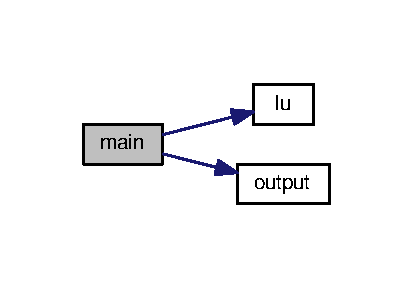
\includegraphics[width=198pt]{LUDecomp_8cpp_a3c04138a5bfe5d72780bb7e82a18e627_cgraph}
\end{center}
\end{figure}


\index{L\+U\+Decomp.\+cpp@{L\+U\+Decomp.\+cpp}!output@{output}}
\index{output@{output}!L\+U\+Decomp.\+cpp@{L\+U\+Decomp.\+cpp}}
\subsubsection[{\texorpdfstring{output(float x[][10], int n)}{output(float x[][10], int n)}}]{\setlength{\rightskip}{0pt plus 5cm}void output (
\begin{DoxyParamCaption}
\item[{float}]{x\mbox{[}$\,$\mbox{]}\mbox{[}10\mbox{]}, }
\item[{int}]{n}
\end{DoxyParamCaption}
)}\hypertarget{LUDecomp_8cpp_a03c4f4fac92a1c3266ad7002a68b4610}{}\label{LUDecomp_8cpp_a03c4f4fac92a1c3266ad7002a68b4610}

\begin{DoxyCode}
65 \{
66     \textcolor{keywordtype}{int} i = 0, j = 0;
67     \textcolor{keywordflow}{for} (i = 0; i < n; i++)
68     \{
69         \textcolor{keywordflow}{for} (j = 0; j < n; j++)
70         \{
71             printf(\textcolor{stringliteral}{"%f "}, x[i][j]);
72         \}
73         cout << \textcolor{stringliteral}{"\(\backslash\)n"};
74     \}
75 \}\end{DoxyCode}

%--- End generated contents ---

% Index
\backmatter
\newpage
\phantomsection
\clearemptydoublepage
\addcontentsline{toc}{chapter}{Index}
\printindex

\end{document}
